\section{Aufbau und Organisation des Projektordners}

\begin{figure}[htbp]
    \centering
      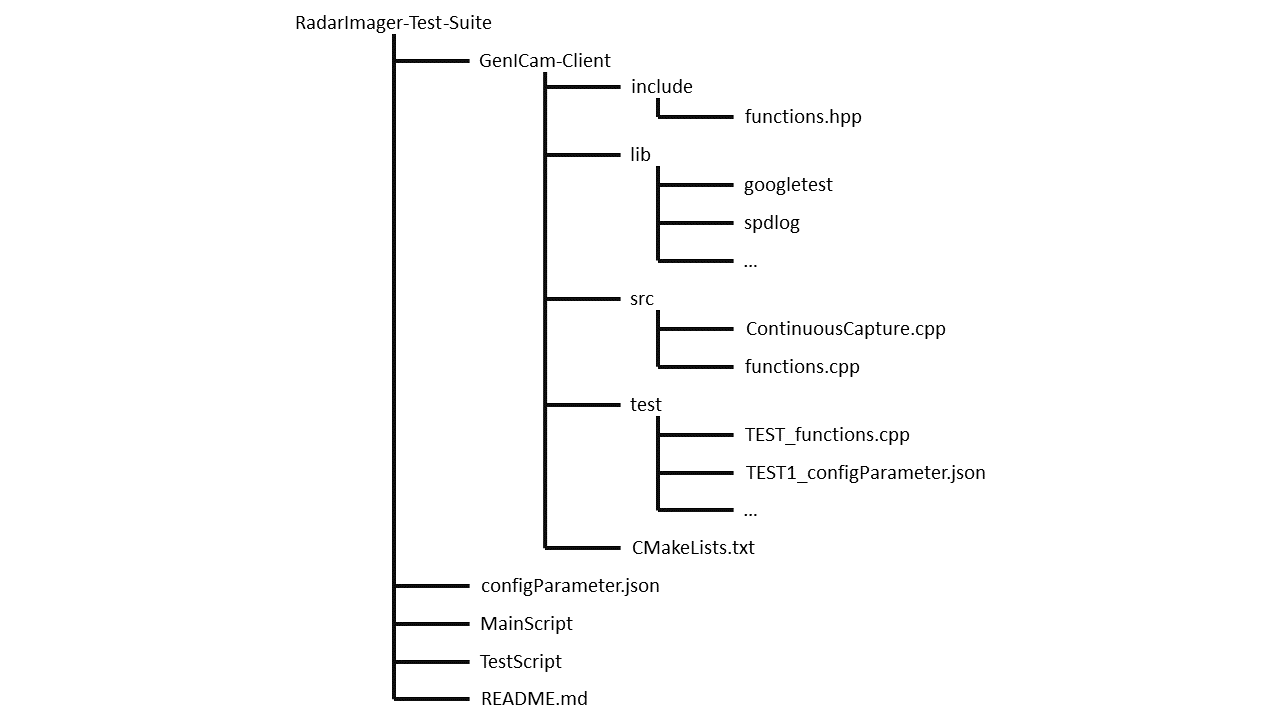
\includegraphics [width=1\textwidth]{Projektstruktur.png}
    \caption[Verzeichnisstruktur]{Verzeichnisstruktur (eigene Darstellung)}
    \label{fig:Verzeichnisstruktur}
\end{figure}

Die Struktur des Testprogramms für den RadarImager ist durch mehrere Unterverzeichnisse klar und logisch aufgebaut. Im Rahmen dieser Projektarbeit liegt der Fokus auf dem 
Verzeichnis \glqq GenICam-Client\grqq. Die Konfigurationsdatei \glqq configParameter.json\grqq\ befindet sich im Hauptordner des Projekts, da sie codeübergreifend 
verwendet wird. Die Ordner \glqq MainScript\grqq\ und \glqq TestScript\grqq, die unter anderem Python-Skripte zur Steuerung des Hardware-Triggers enthalten, sind für diese Arbeit 
von untergeordneter Bedeutung.

Die Codebasis des GenICam-Clients ist zur besseren Übersicht und Handhabbarkeit in folgende Unterverzeichnisse aufgeteilt:

\begin{itemize}
    \item \textbf{include}: Dieser Ordner enthält die Header-Datei \glqq functions.hpp\grqq, welche die Schnittstellen für die in \glqq src\grqq\ implementierten Klassen und Funktionen deklariert. Zudem sind hier verschiedene Strukturen (structs) definiert.
    \item \textbf{lib}: Hier sind die im Projekt verwendeten Bibliotheken, wie zum Beispiel \glqq spdlog\grqq, abgelegt. Diese Strukturierung unterstützt eine klare Abgrenzung zwischen eigenem Code und externen Bibliotheken.
    \item \textbf{src}: Dieser Ordner enthält den Quellcode des Projekts, einschließlich der Hilfsfunktionen und dem Hauptprogramm zur Verarbeitung der empfangenen Daten.
    \item \textbf{test}: In diesem Verzeichnis befinden sich die Modultests, die zur Überprüfung der Funktionalität des Codes dienen. Es umfasst auch zusätzliche Dateien, die in den Tests verwendet werden.
\end{itemize}

Zur Automatisierung und effizienten Verwaltung des Build-Prozesses wird CMake eingesetzt. CMake erleichtert die Integration und Verwaltung von Abhängigkeiten sowie 
die Konfiguration des Testframeworks, um eine konsistente und fehlerfreie Build-Umgebung zu gewährleisten. Hierzu wird eine CMakeLists.txt-Datei angelegt. 
Diese Datei enthält spezifische Anweisungen, die es CMake ermöglichen, die notwendigen Bibliotheken korrekt zu lokalisieren, einzubinden und mit dem Hauptprojekt zu verknüpfen. 
Dadurch wird sichergestellt, dass alle Komponenten des Projekts nahtlos zusammenarbeiten und die Build-Prozesse reibungslos ablaufen können.

Im Anhang dieser Projektarbeit finden sich die Quellcodedateien \glqq ContinuousCapture.cpp\grqq, \glqq functions.hpp\grqq\ und \glqq functions.cpp\grqq.